\documentclass[tikz]{standalone}
\usepackage{amsmath}
\usepackage{amssymb}
\usepackage{amsfonts}
\usepackage{tikz}

\thispagestyle{empty}
\begin{document}


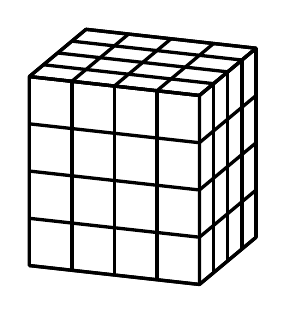
\begin{tikzpicture}[scale=0.6, line join=round, 
x={(.9cm,-.1cm)}, 
y={(0cm,1cm)}, 
z={(.3cm,.25cm)}]

% Draw the front face grid
\foreach \x in {0,...,4} {
	\draw[very thick] (\x,0,0) -- (\x,4,0); % vertical lines
}
\foreach \y in {0,...,4} {
	\draw[very thick] (0,\y,0) -- (4,\y,0); % horizontal lines
}

% Draw the right face grid
\foreach \y in {0,...,4} {
	\draw[very thick] (4,\y,0) -- (4,\y,4); % verticals
}
\foreach \z in {0,...,4} {
	\draw[very thick] (4,0,\z) -- (4,4,\z); % depth lines
}

% Draw the top face grid
\foreach \x in {0,...,4} {
	\draw[very thick] (\x,4,0) -- (\x,4,4); % verticals on top face
}
\foreach \z in {0,...,4} {
	\draw[very thick] (0,4,\z) -- (4,4,\z); % horizontal depth lines
}

% Draw cube outline
\draw[very thick] (0,0,0) -- (4,0,0) -- (4,4,0) -- (0,4,0) -- cycle; % front face
\draw[very thick] (4,0,0) -- (4,0,4) -- (4,4,4) -- (4,4,0);          % right face
\draw[very thick] (0,4,0) -- (0,4,4) -- (4,4,4);                     % top face outline

\end{tikzpicture}

\end{document}
